
\color{Navy} % Navy color for the abstract

\begin{abstract}
The heavy quark doublet plays a central role in the quest for new physics. The complementarity between studies of electroweak top quark production and bottom quark production is therefore intuitively clear and pointed out in the literature.
The tension between the LEP measurement and the Standard Model prediction of the forward-backward asymmetry \afb\ is still one of the unsolved questions in the field and may be interpreted as a first manifestation of New Physics in the heavy quark sector. The process $e^+e^-\to b\bar{b}$ at the ILC offers a unique opportunity for a final word on the tension. Polarised beams allow for a large disentangling of the coupling constants or form factors that govern the $Z^0/\gamma b \bar{b}$ vertex.

%This poster presents a detailed simulation study of the process $e^+e^-\to b\bar{b}$ at 250\,GeV with the ILD Detector. Besides the phenomenological implications, the studies demonstrate that with a careful analysis of the final state the charge of the b-quarks can be determined on an event-by-event basis with the ILD Detector. Such a capability is unprecedented by past and present particle physics experiments.
\end{abstract}

%----------------------------------------------------------------------------------------
%	INTRODUCTION
%----------------------------------------------------------------------------------------

\color{DarkSlateGray} % SaddleBrown color for the introduction

\setlength{\columnsep}{20pt}%
\begin{wrapfigure}{r}{0.20\textwidth}
	%\centering
	
	\hspace{1.5cm}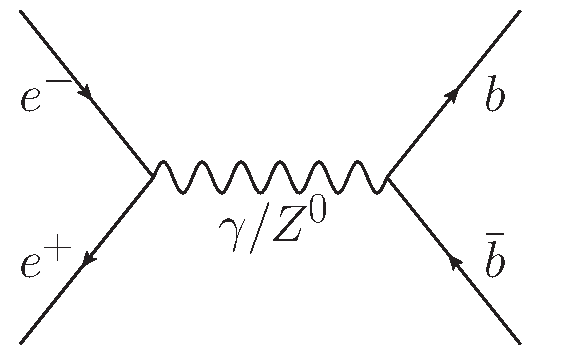
\includegraphics[width=0.18\textwidth]{figures/bbbar.pdf}
	%\caption{\sl The leading order Feynman diagram of the $e^+ e^-\to b\bar{b}$ channel.}
	\label{fig:bbbar}
	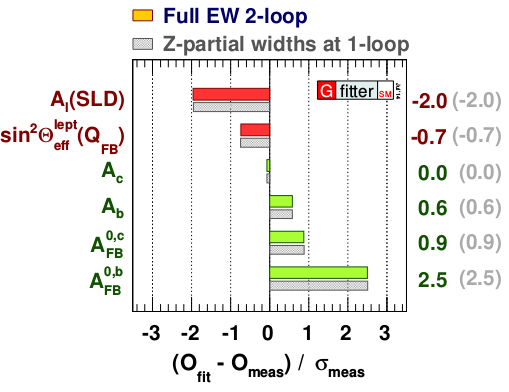
\includegraphics[width=0.20\textwidth]{figures/deviation.png}
	\caption{\sl Feynman diagram and the results of the electroweak fit for (among others) \afb\ and $A_l(SLD)$~\cite{bib:AfbSMFit}.}
	\label{fig:deviation}
\end{wrapfigure}

\section*{Introduction}

%So far, LEP~I has determined the b-quark couplings to the $Z^0$ boson by measuring the b partial width and the forward-backward asymmetry called \afb. These quantities provide the most precise value of $\sin^2\theta_W$ at LEP~I. It turns out that this value is at about three standard deviation away from the very precise value from SLD using beam polarization~\cite{bib:AfbSMFit}. Redoing precisely this measurement is therefore a priority for future $e^+e^-$ colliders. 


%In this study, we intend to prove that the International Linear Collider~\cite{bib:ILC}, with \textbf{polarized beams and high luminosity}, offers a unique opportunity for precise measurements well above the resonance, where both $Z^0$ and photon exchanges are present. 
%This additional complexity may turn up to be of a great advantage since it allows, through $\gamma - Z^0$ interference, to be sensitive to the sign of $Z^0$ couplings and fully solve the LEP~I puzzle in an unambiguous way. 
%Recall that the LEP~I anomaly can be interpreted up to a sign ambiguity for what concerns the right‐handed coupling $Z^0 b\bar{b}$, referred hereafter as $g_R^Z$, which shows the largest deviation~\cite{bib:RSTOP}.  

%\begin{center}\vspace{1cm}
%	\label{fig:ILCScheme}
%	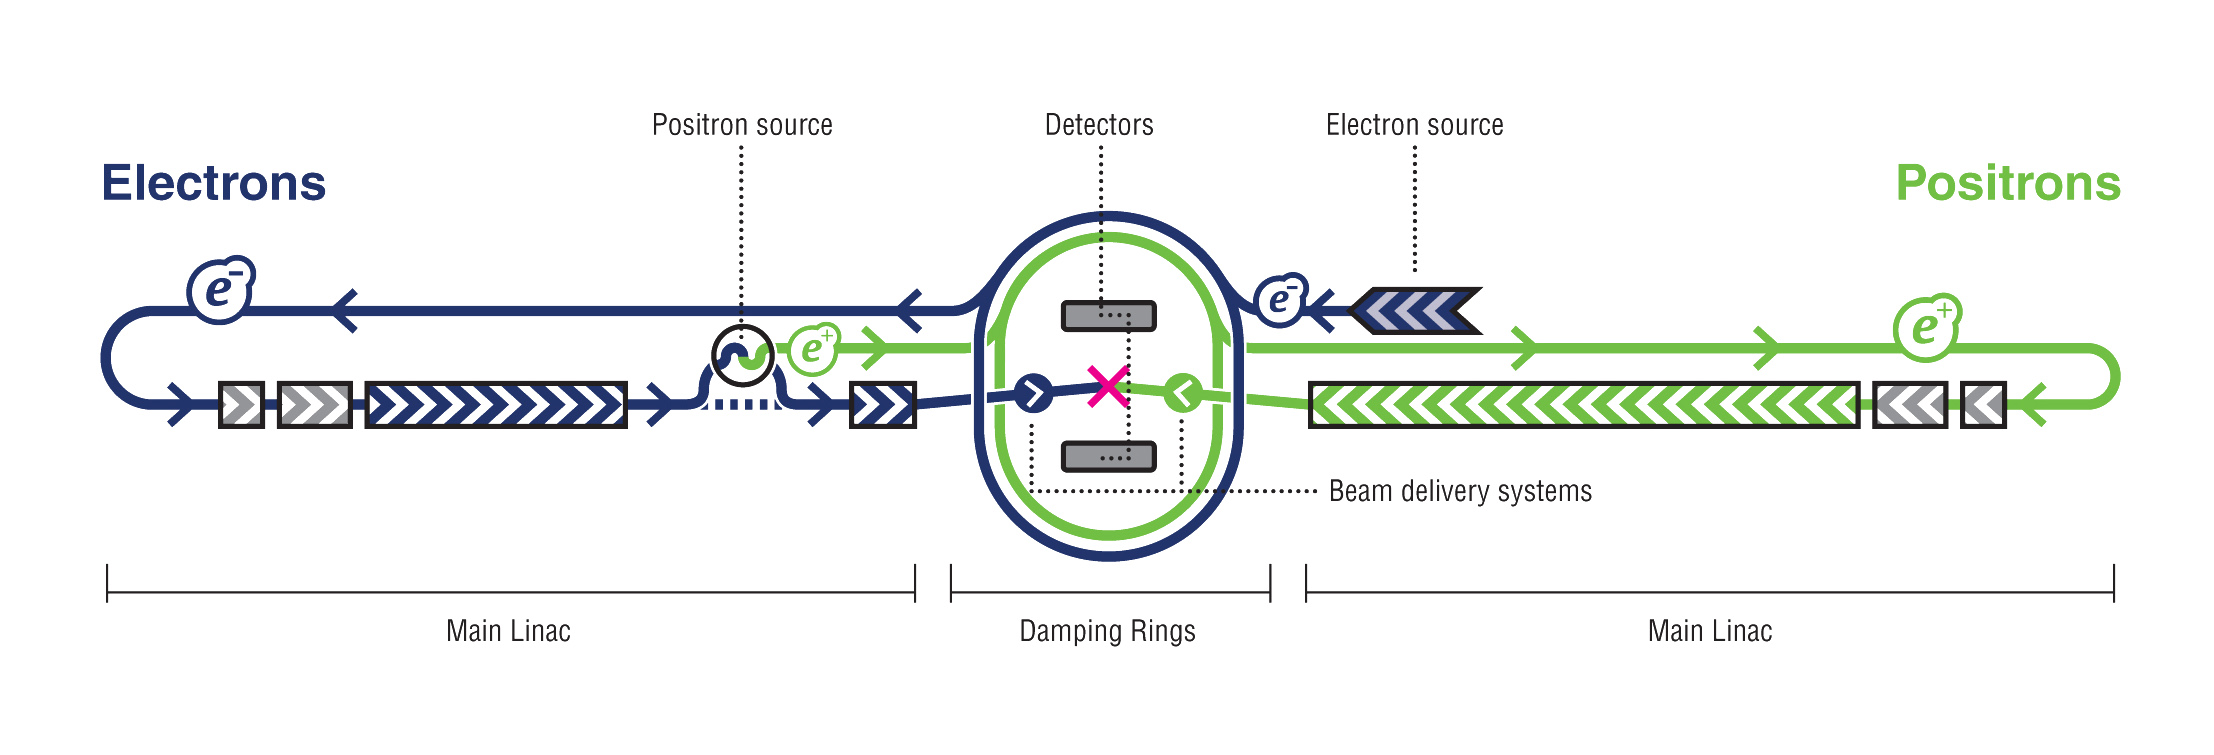
\includegraphics[width=0.95\linewidth]{../graphics/ILC_scheme.jpg}
%	\captionof{figure}{ \sl Schematic view of the ILC accelerator complex. }
%\end{center}\vspace{1cm}
%\color{Blue} The $e^+ e^-\to b\bar{b}$ channel is studied at $\sqrt{s}=250$\,GeV using full simulation of the ILD experiment.
%\color{DarkSlateGray} The high-granularity of the ILD subdetectors allows for an individual particle reconstruction using the Particle Flow approach.
%The schematic view of the ILD concept and the subdetector layout is presented in Fig.~\ref{fig:ILDScheme}.

%The Vertex Detector (VXD) has 3 double layers with about $3\,\mu$m  resolution on the track impact parameters.  
%The vertex reconstruction algorithms are able to separate the secondary and tertiary vertices from b-hadrons.

%This enables a highly efficient b- and c-tagging of the jets and a detailed b-hadron vertex reconstruction. 
%The central tracker of the ILD detector is Time Projection Chamber (TPC), which will provide up to 224 points per track allowing for $dE/dx$-based particle identification.


%The main goal of the study is to reconstruct the b-quark polar angle distributions for both beam polarization cases at the ILC. From that, the precision on the b-quark electroweak couplings is determined and compared to the LEP~I results. 


\begin{itemize}
	\item So far, LEP~I has determined the b-quark couplings to the $Z^0$ boson by measuring the b partial width and the forward-backward asymmetry called \afb.
	\item It turns out that this value is at about three standard deviation away from the very precise value from SLD using beam polarization~\cite{bib:AfbSMFit} and may be caused by New Physics~\cite{bib:RSTOP}.
	\item Redoing precisely the b-quark electroweak coupling measurement is therefore a priority for future $e^+e^-$ colliders. 
	
\end{itemize}

\begin{itemize}
	
	\item In this study, we intend to prove that the International Linear Collider~\cite{bib:ILC}, with \textbf{polarized beams and high luminosity}, offers a unique opportunity for precise measurements well above the resonance, where both $Z^0$ and photon exchanges are present. 
	\item {\color{Blue} The $e^+ e^-\to b\bar{b}$ channel is studied at $\sqrt{s}=250$\,GeV using full simulation of the ILD experiment at the ILC.}
	%\vspace{2cm}
	\item The high-granularity of the ILD subdetectors allows for an individual particle reconstruction using the Particle Flow approach.
	%\item The main goal of the study is to reconstruct the b-quark polar angle distributions for both beam polarization cases at the ILC. From that, the precision on the b-quark electroweak couplings is determined and compared to the LEP~I results. 
\end{itemize}


\begin{center}\vspace{1.8cm}
	\centering
	
	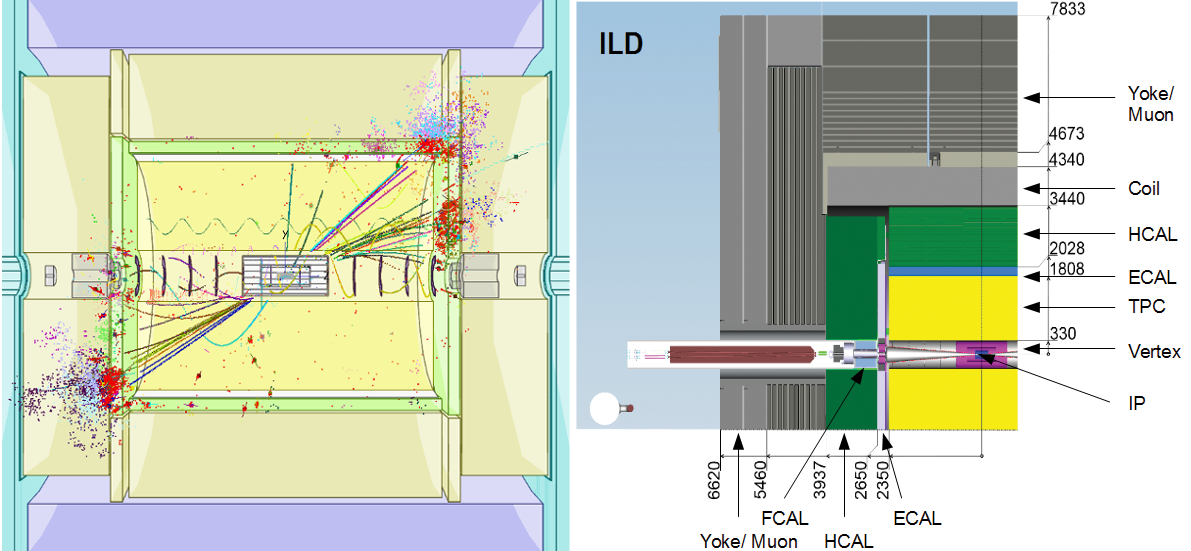
\includegraphics[width=0.9\linewidth]{figures/ild3.png}
	\captionof{figure}{ \sl Event display of the $e^+ e^-\to b\bar{b}$ process in a full simulation of the ILD detector (left) and schematic view of the ILD concept~\cite{bib:ILC} (right). }
	\label{fig:ILDScheme}
\end{center}\vspace{1cm}
%----------------------------------------------------------------------------------------
%	OBJECTIVES
%----------------------------------------------------------------------------------------

\color{DarkSlateGray} % DarkSlateGray color for the rest of the content

\section*{B-quark charge measurement}
\setlength{\columnsep}{20pt}%
\begin{wrapfigure}{R}{0.22\textwidth}
	%\centering
	
	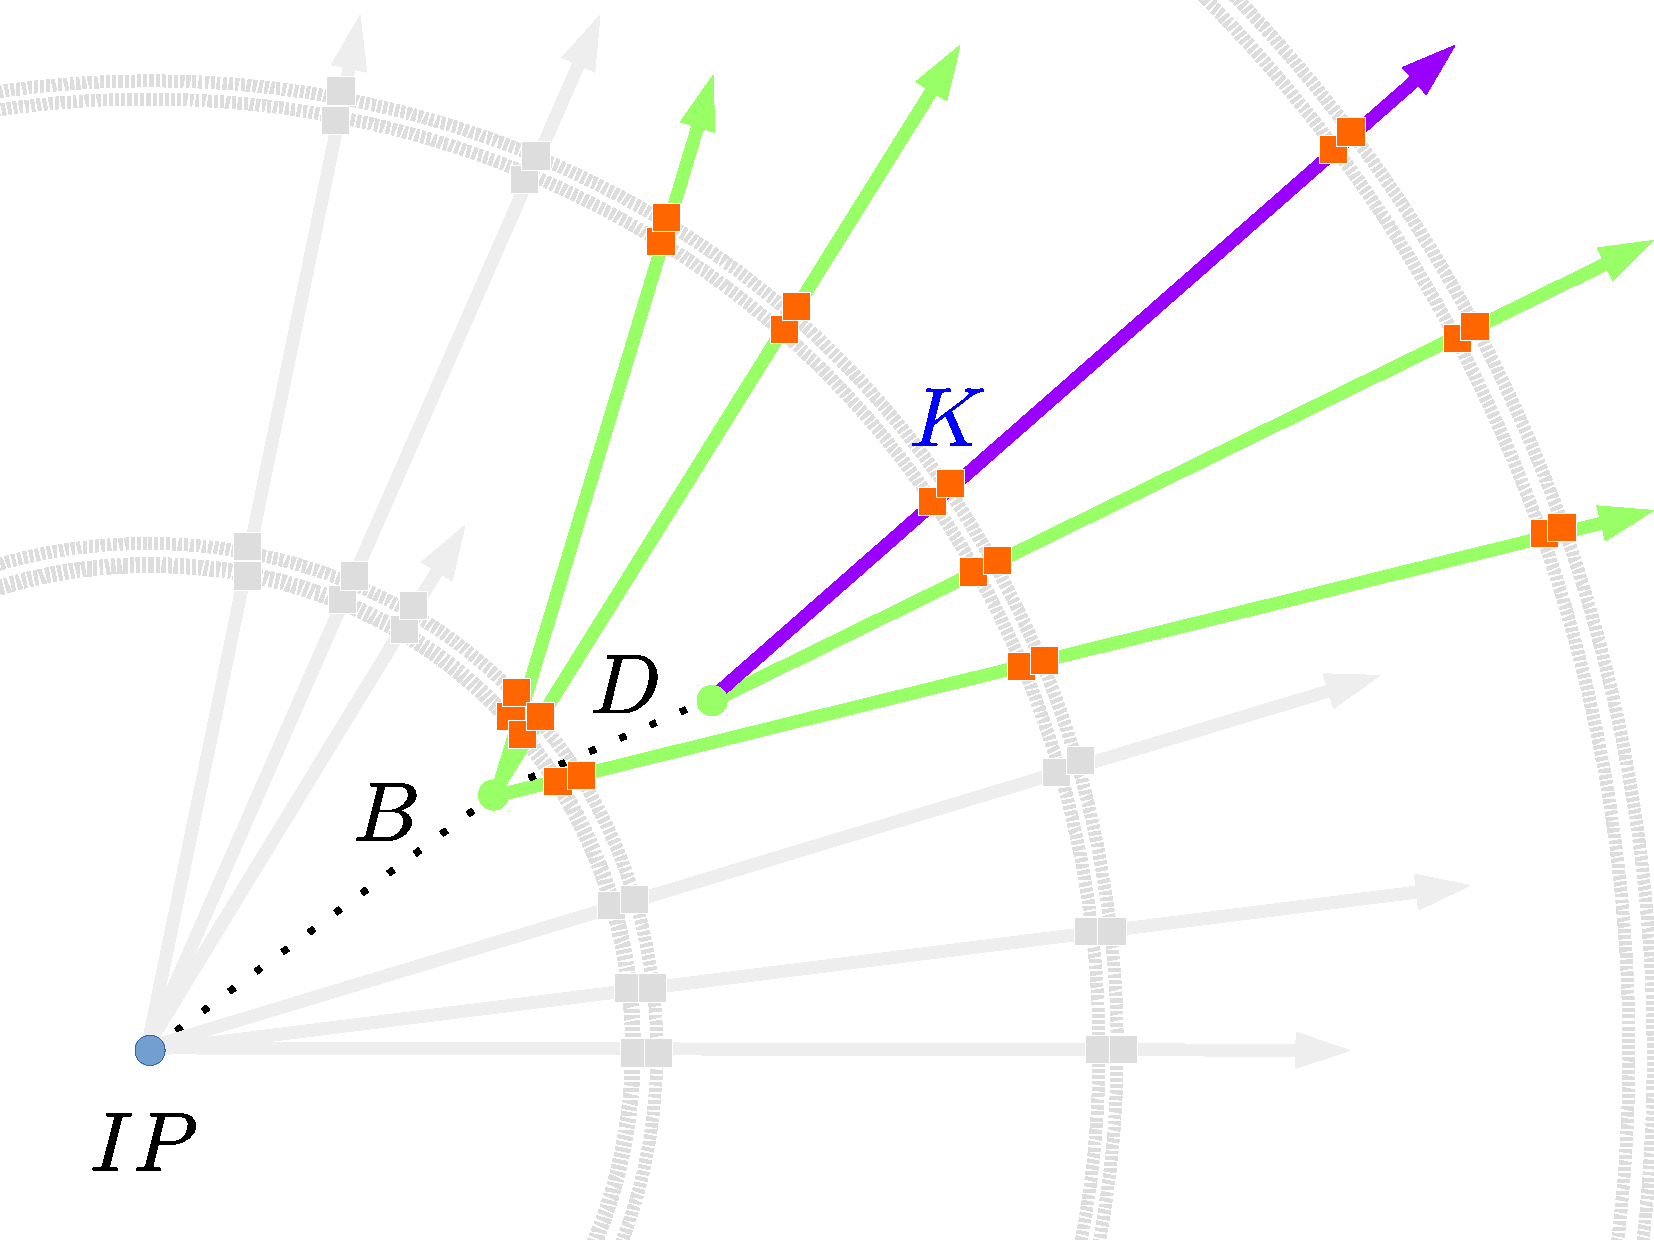
\includegraphics[width=0.22\textwidth]{figures/vtx.pdf}
	\caption{\sl B-hadron vertices.}
	\label{fig:vtx}

\end{wrapfigure}

\color{Blue}
The b-quark polar angle reconstruction requires an accurate b-quark charge measurement. 
The b-quark charge is identified using two basic signatures:
\begin{itemize}
	\item \textbf{Vertex charge} is a sum of all reconstructed particles charges, which are associated to the b-hadron vertices. 
	\item \textbf{Kaon charge} is a charge of kaons found in b-hadron vertices. 
\end{itemize}

\color{DarkSlateGray}
%Sometimes, the vertex reconstruction algorithms may fail and lose one or several particles from the reconstructed b-hadron vertices. This leads to a wrong vertex charge measurement. 
%The reasons behind the missing b-hadron particles are connected to reconstruction shortcomings or to a low momentum or a low offset of the b-hadron particles. 
The developed Vertex Charge Recovery procedure enhances the vertex charge purity by adding the missing particles back to the reconstructed vertices. 


The kaon identification is possible using the TPC $dE/dx$ information. After equalizing the $dE/dx$ in angular spectrum, the kaons from b-hadron vertices can be identified with 97.\% purity and 87\% efficiency.
% However, the $B-\bar{B}$ oscillations will degrade the kaon charge signature purity for $B^0$ mesons.
\begin{center}\vspace{0.5cm}
	
	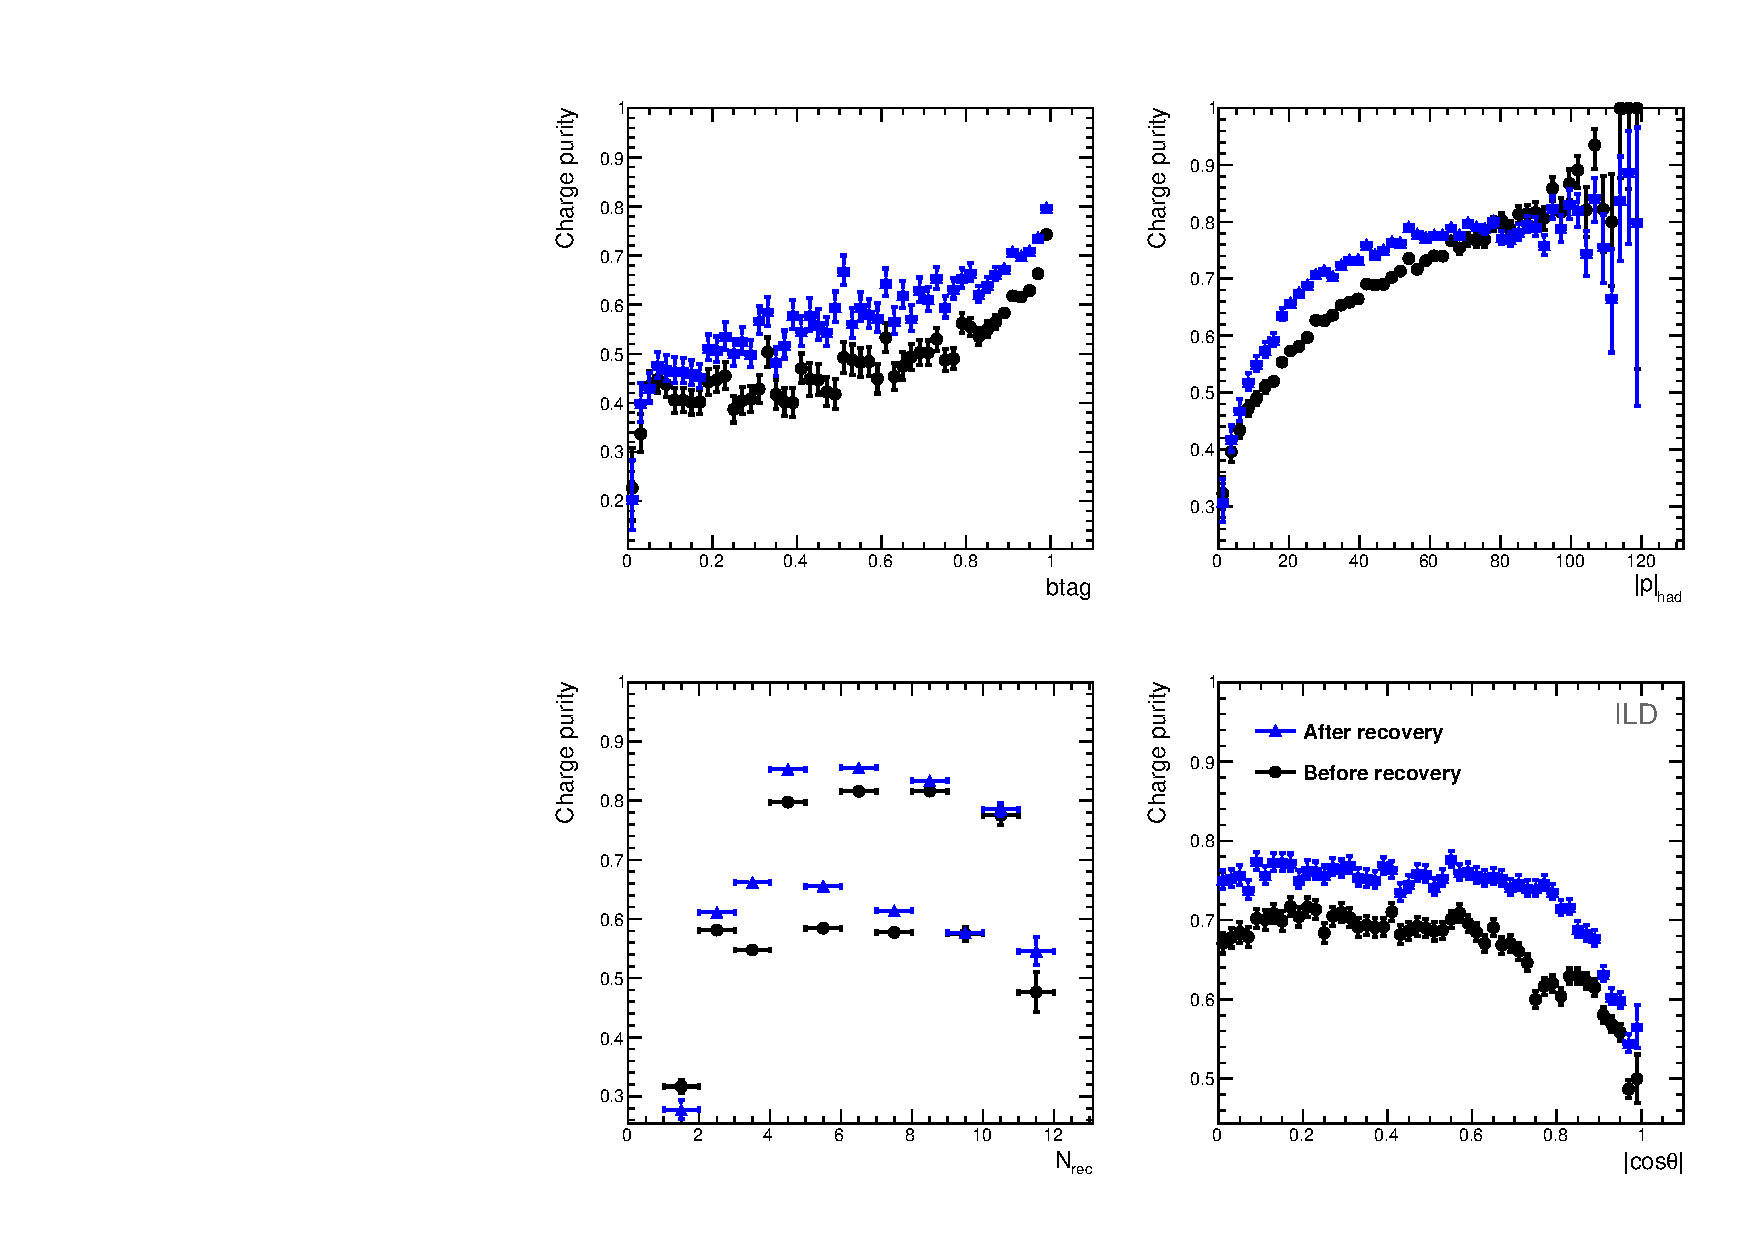
\includegraphics[clip, trim=10cm 0cm 0cm 10cm,width=0.45\linewidth]{plots/purity-recovery-ild.pdf}\label{fig:Charges_a_3}
	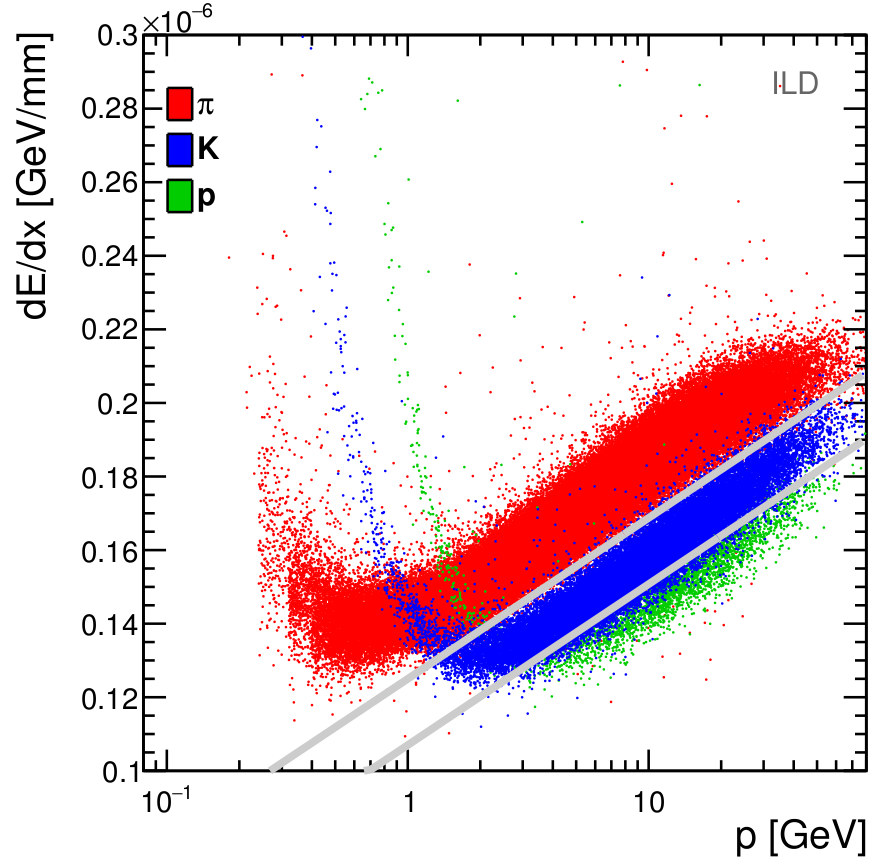
\includegraphics[width=0.41\linewidth]{plots/dedx2.png}\label{fig:Charges_b_3}
	\captionof{figure}{\sl Vertex charge purity as function of $\cos\theta$ (left) and energy deposition per unit of length $dE/dx$ as function of particle momentum $p$ (right).}
	\label{fig:Charges_3}
\end{center}\vspace{1cm}
%The plots of the vertex charge purity and the $dE/dx$ as function of particle momentum for different hadrons are shown in Fig.~\ref{fig:Charges_3}.



%------------------------------------------------

%----------------------------------------------------------------------------------------
%	POLAR ANGLE 
%----------------------------------------------------------------------------------------

\section*{B-quark polar angle spectrum}

%The reconstructed b-quark polar angle distributions at $\sqrt{s} = 250$\,GeV using a combination of kaon and vertex charge signatures are demonstrated in Fig.~\ref{fig:BAsymmetryFinal_3}. The integrated luminosity $\mathcal{L}_I = 250$\,fb$^{-1}$ is assumed for each beam polarization.
The reconstructed b-quark polar angle distributions at $\sqrt{s} = 250$\,GeV and $e^-_L, e^+_R = \pm1, \mp1$ and $\mathcal{L} = 2\cdot 250 $\,fb$^{-1}$.
\begin{center}\vspace{0.5cm}

	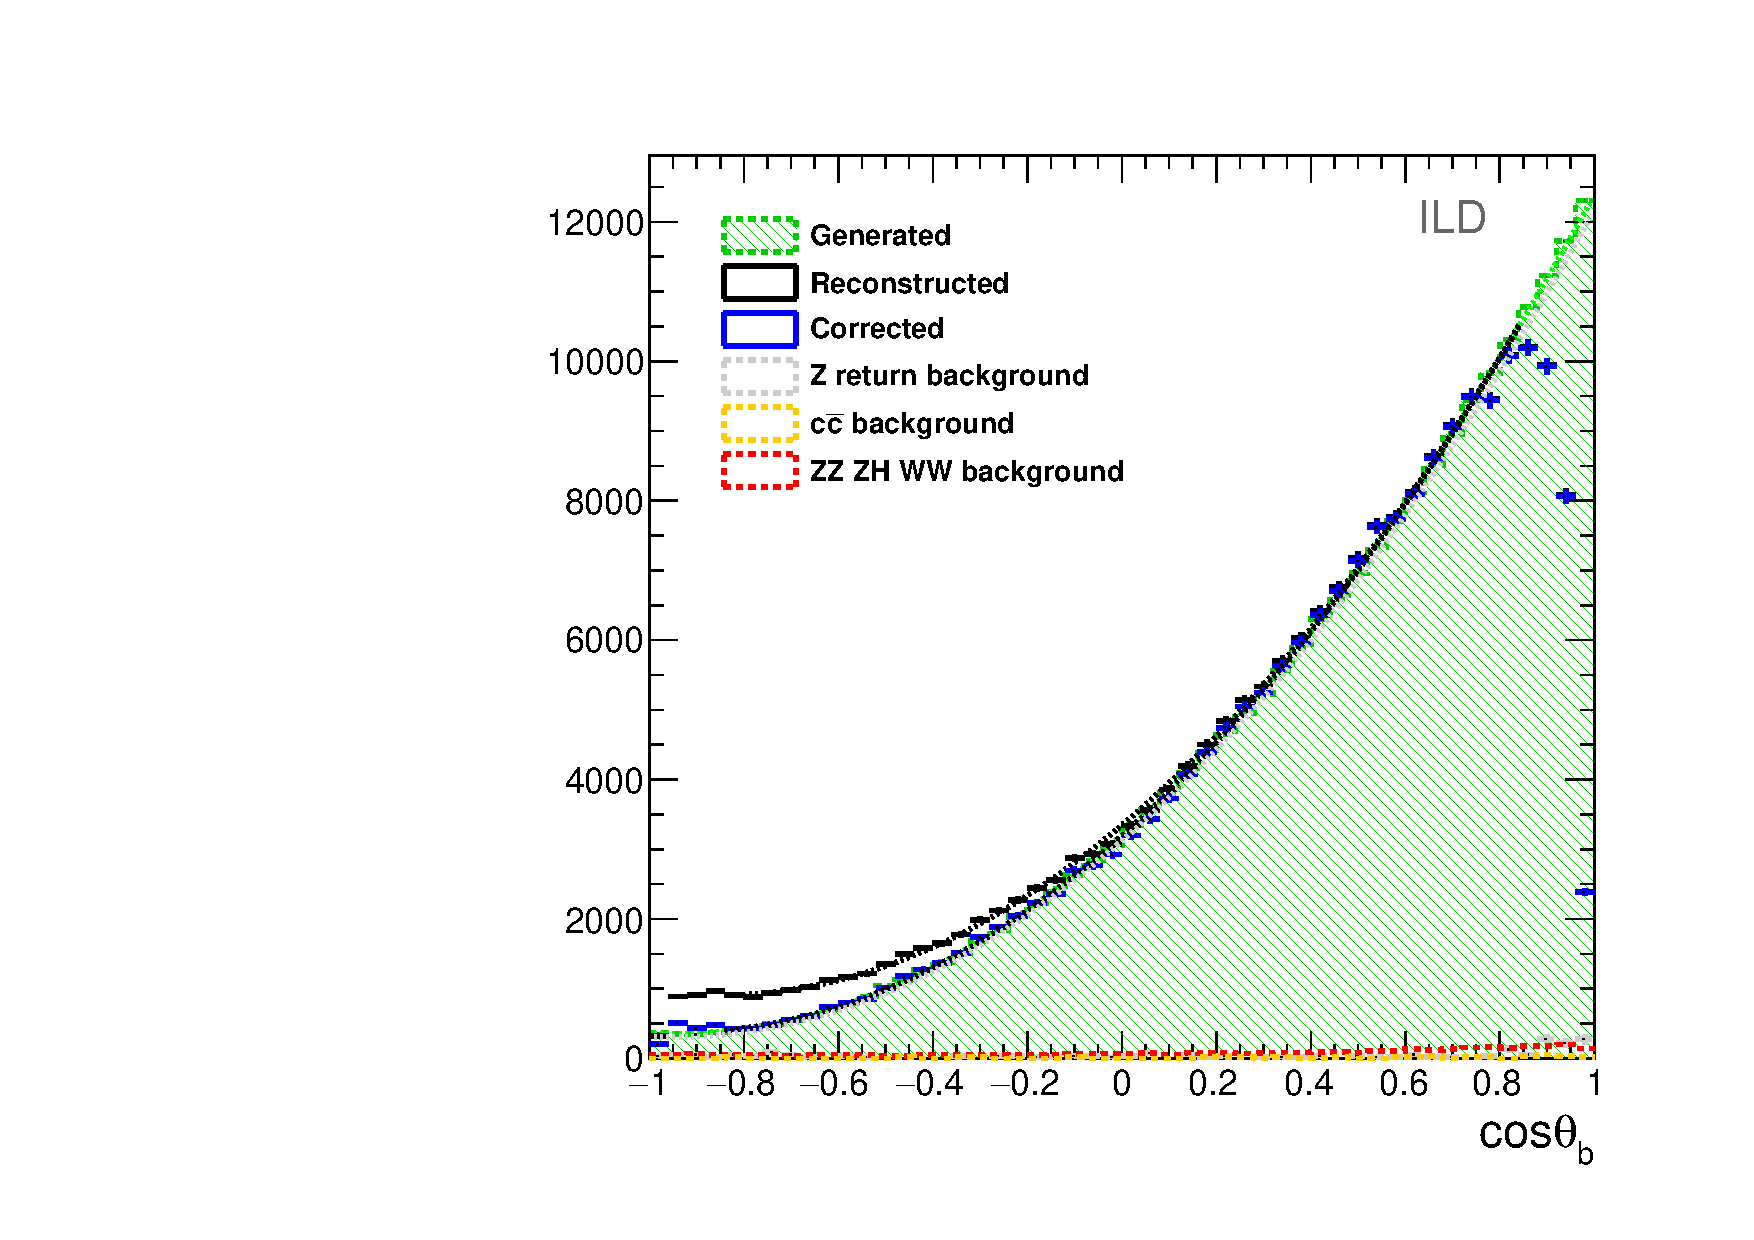
\includegraphics[width=0.45\linewidth]{plots/basymmetry-left-ild.pdf}
	\llap{\shortstack{%
			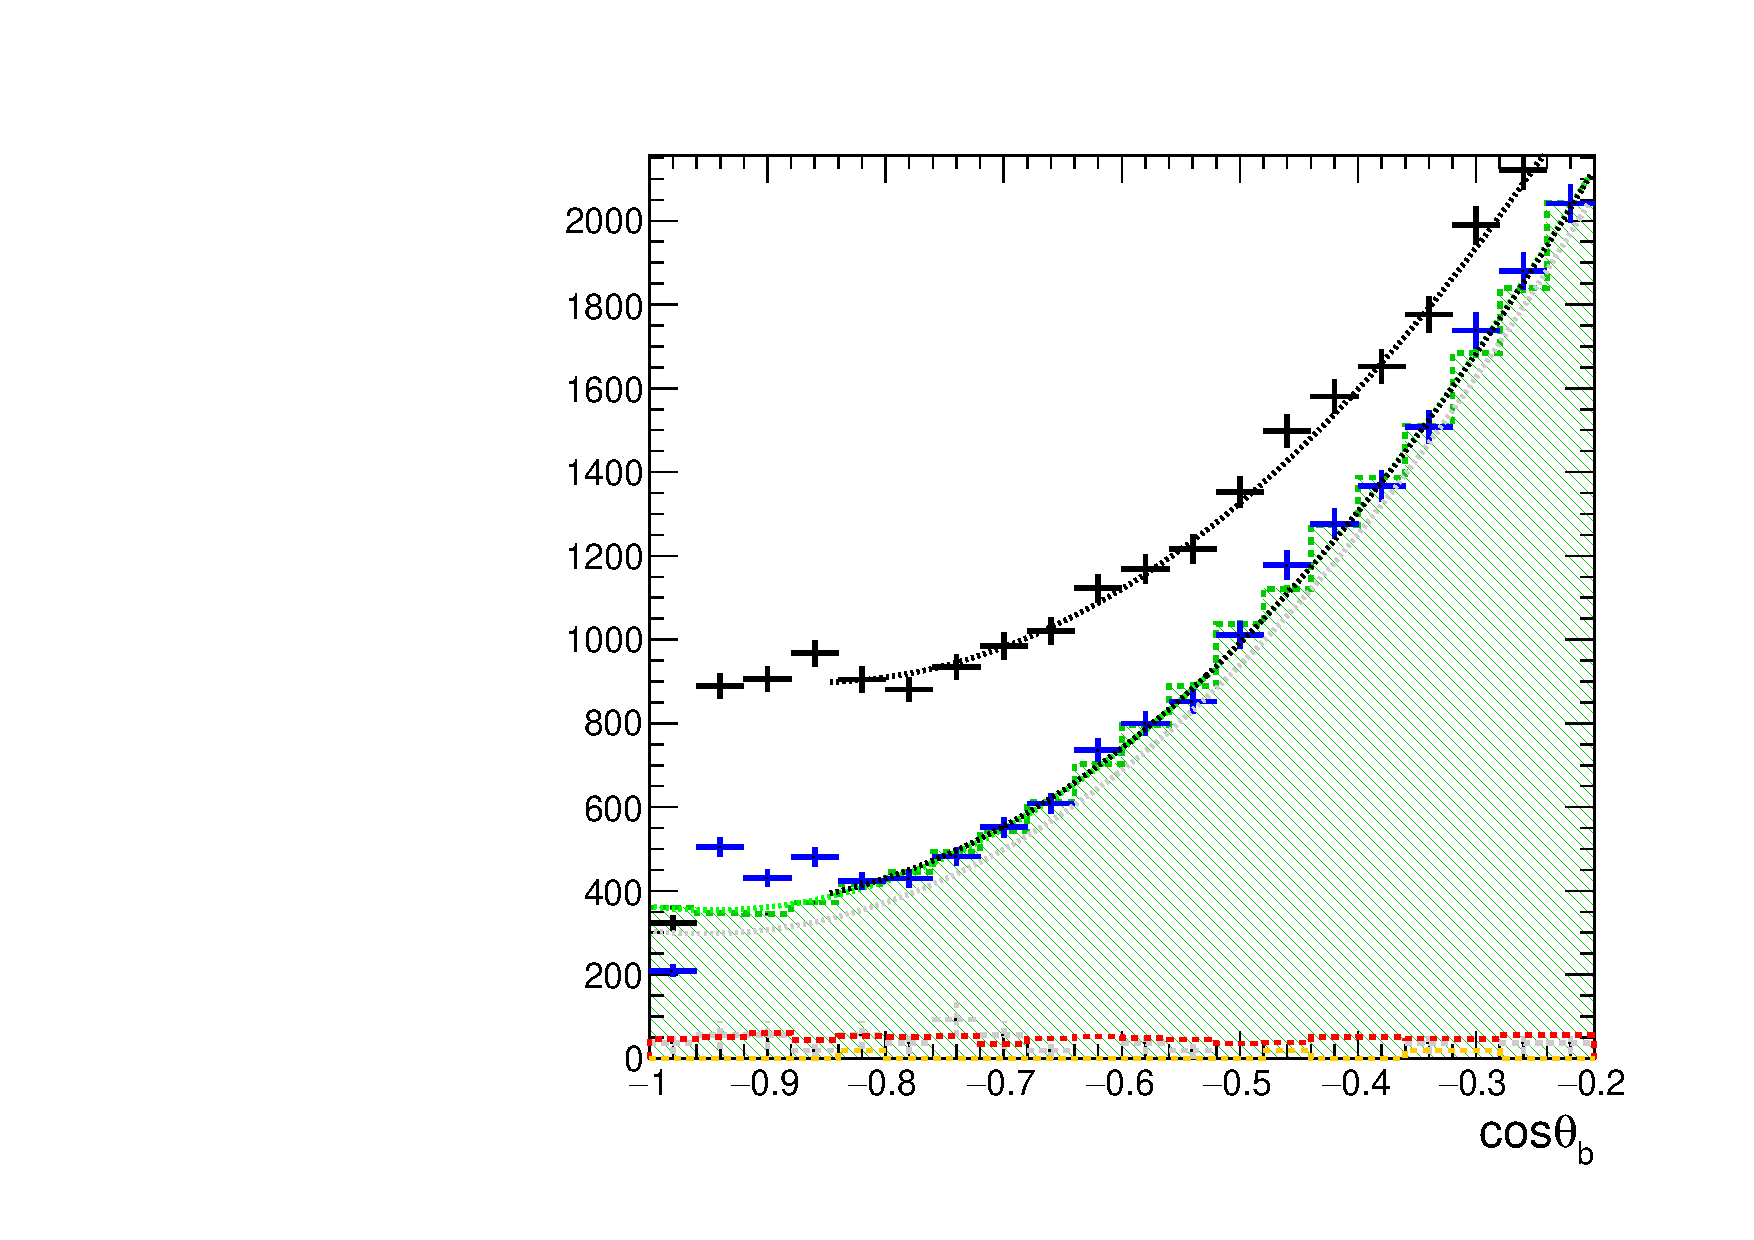
\includegraphics[clip, trim=0cm 0cm 1.3cm 1.3cm, scale=.3]{../ILD/plots/zoom-final.pdf}\\
			\rule{0ex}{1.2in}%
		}
		\rule{4.1in}{0ex}}
	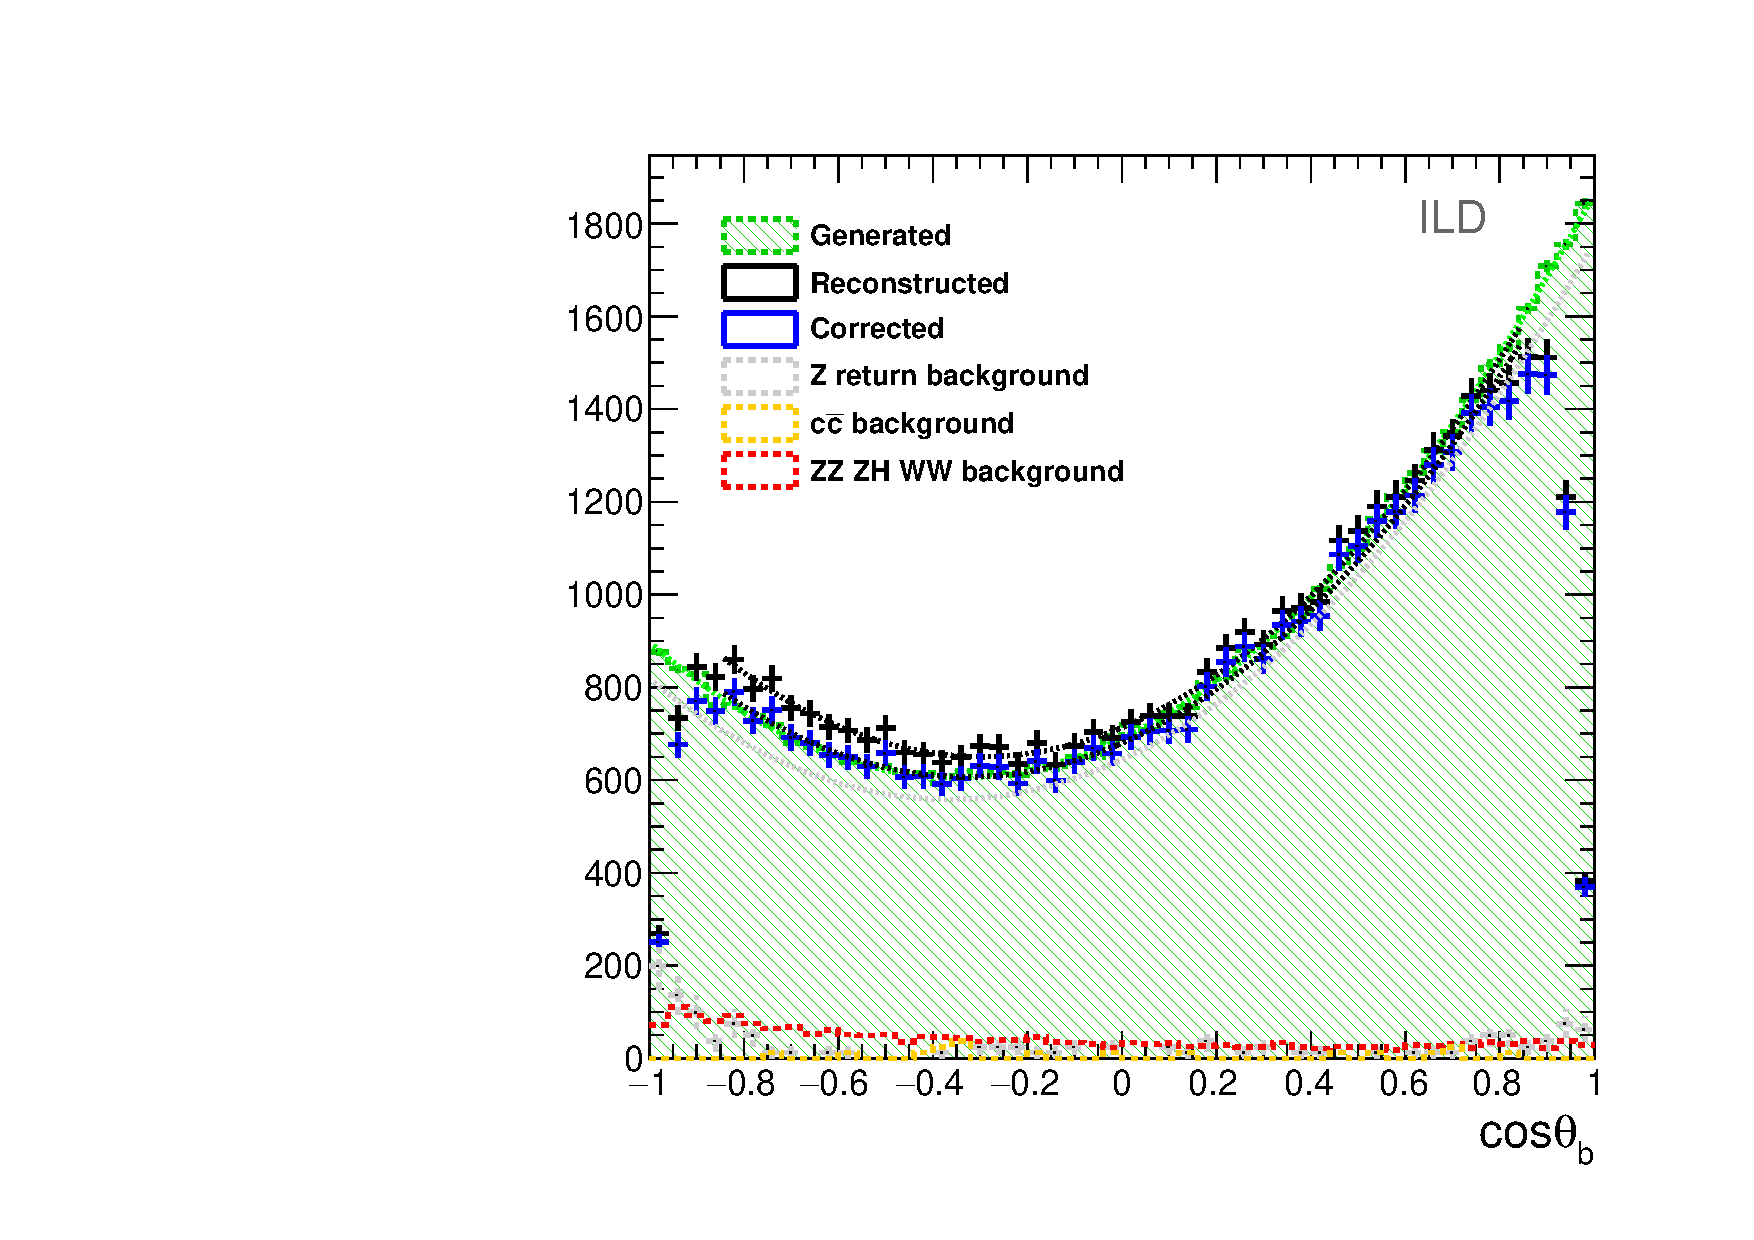
\includegraphics[width=0.45\linewidth]{plots/basymmetry-right-ild.pdf}
	\captionof{figure}{ \sl Generated b-quark polar angle distribution compared to the final reconstructed b-quarks polar angle in left-handed case (left) and right-handed polarization case (right) with overlaid background processes.
	The distributions are fitted by the general cross section function, defined as ${\color{Blue}	S (1+\cos^2\theta) + A \cos\theta}$. The extracted paramters are rescaled to the realistic polarization $e^-_L, e^+_R = \pm0.8, \mp0.3$ and the luminosity sharing of the ILC physics program. }
		\label{fig:BAsymmetryFinal_3}
\end{center}\vspace{0.5cm}

%The kaon and vertex charge purity is defined using the measured events with misreconstructed charges. Using the measured purities, the reconstructed spectrum is corrected using a data-driven procedure.
%The background contribution is small. 


\section*{Interpretation}

%The relative precisions on the $Z^0b\bar{b}$ couplings, $g_L^Z$ and $g_R^Z$, for the LEP~I measurements and for the expected ILC performance are shown in Fig.~\ref{fig:LEPILCResult_3}. 
The ILC precision on the $g_R^Z$ coupling is enough to fully confirm or discard the New Physics influence on the b-quark electroweak couplings. 
\begin{center}\vspace{0.5cm}
	
	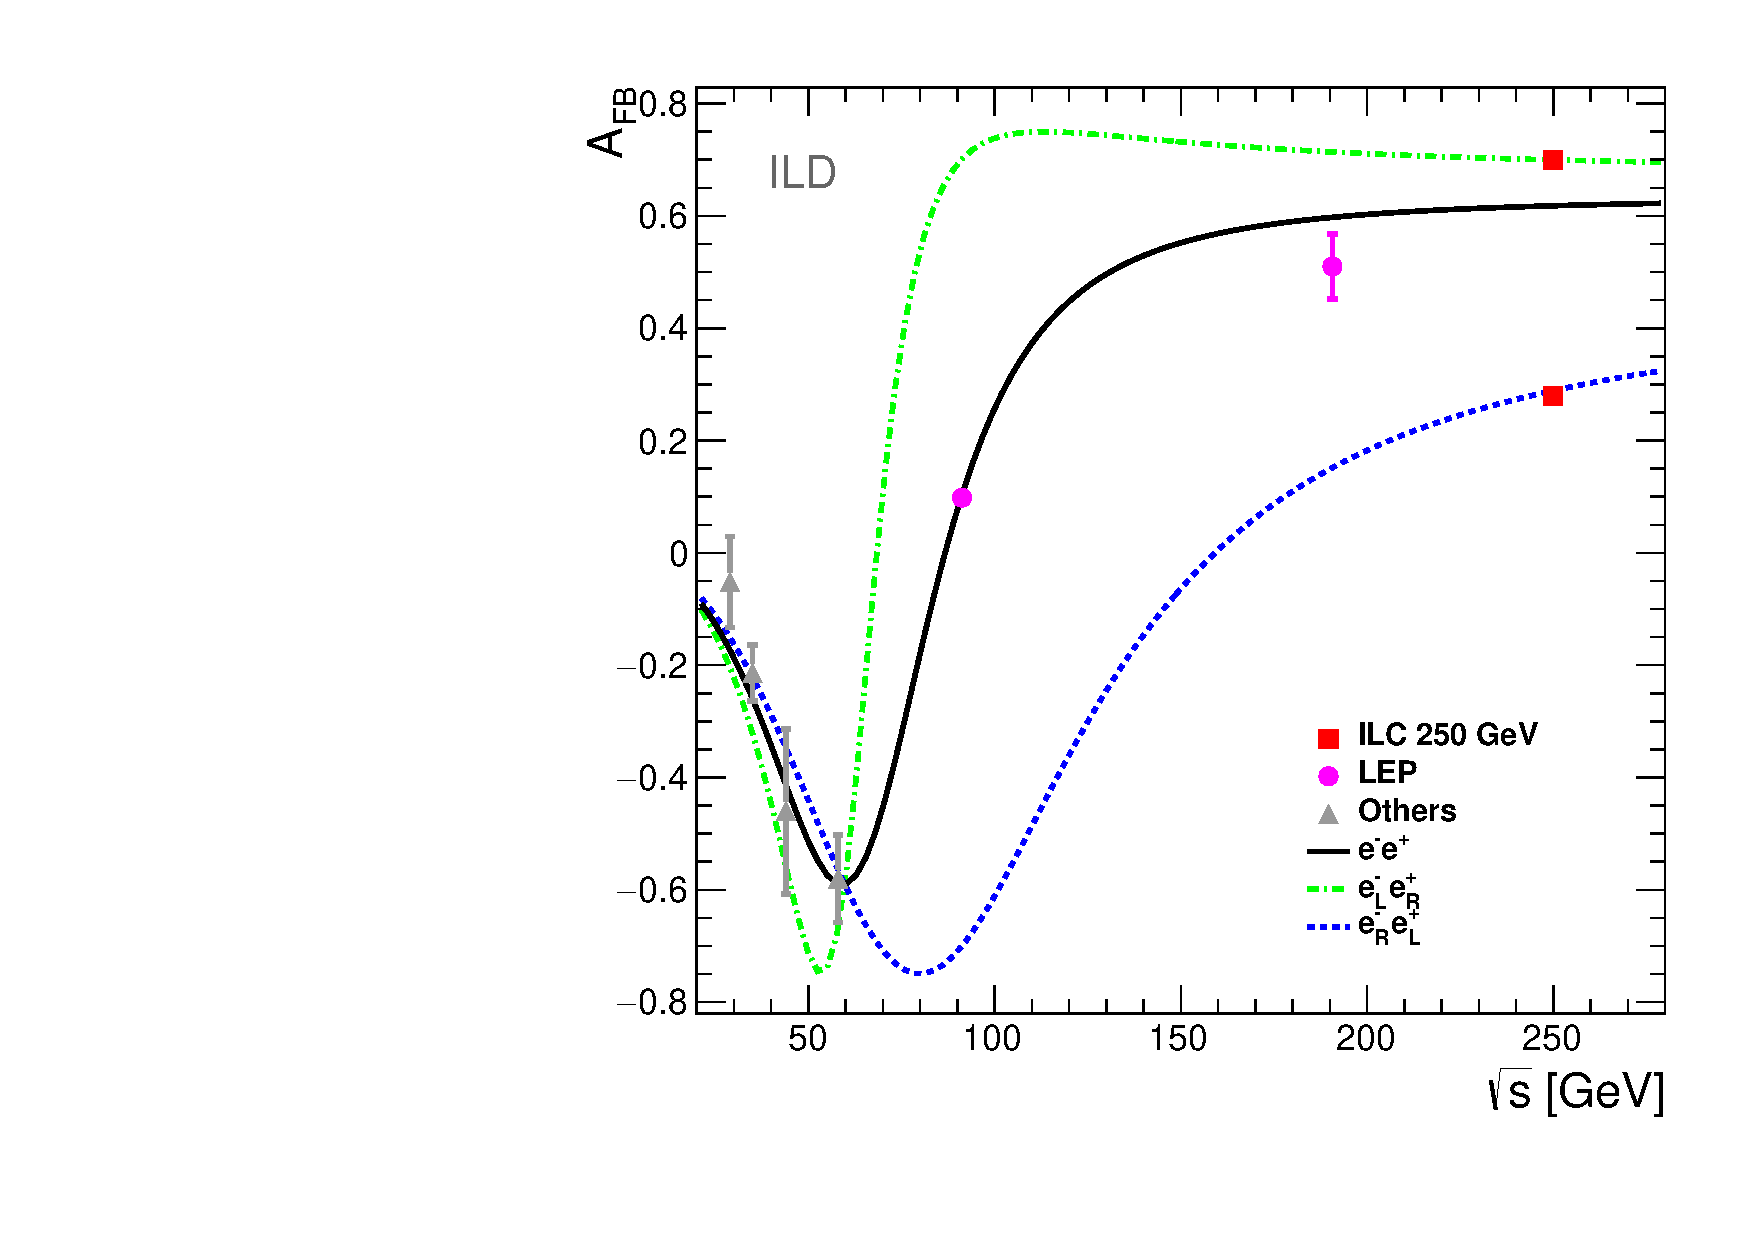
\includegraphics[width=0.45\linewidth]{plots/afb-sqrts.pdf}
	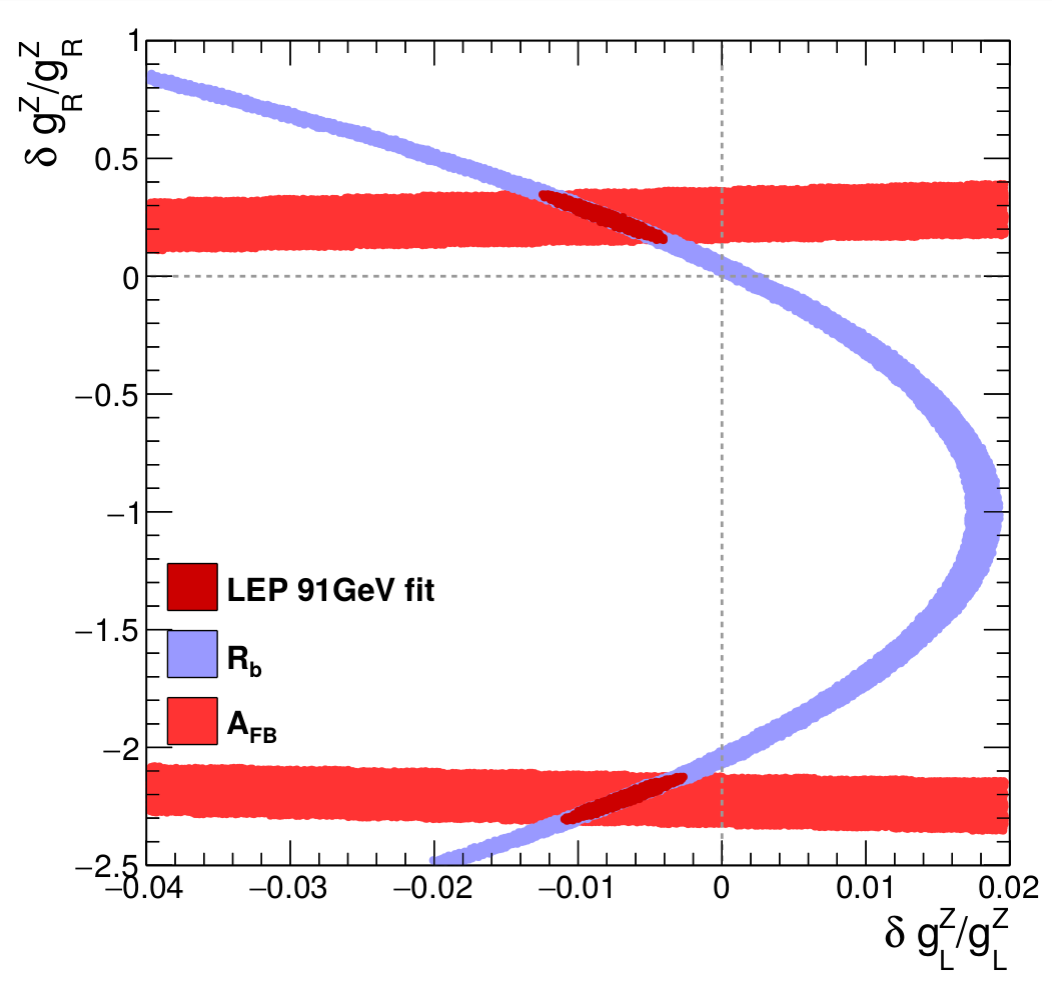
\includegraphics[width=0.45\linewidth]{plots/lep-result-full.png}\\
	%\captionof{figure}{ Comparison of the LEP measurements to the expected precision at the ILC.}
	%\label{fig:LEPILCResult_3}
%\end{center}\vspace{0.5cm}
%\begin{center}\vspace{0.5cm}

	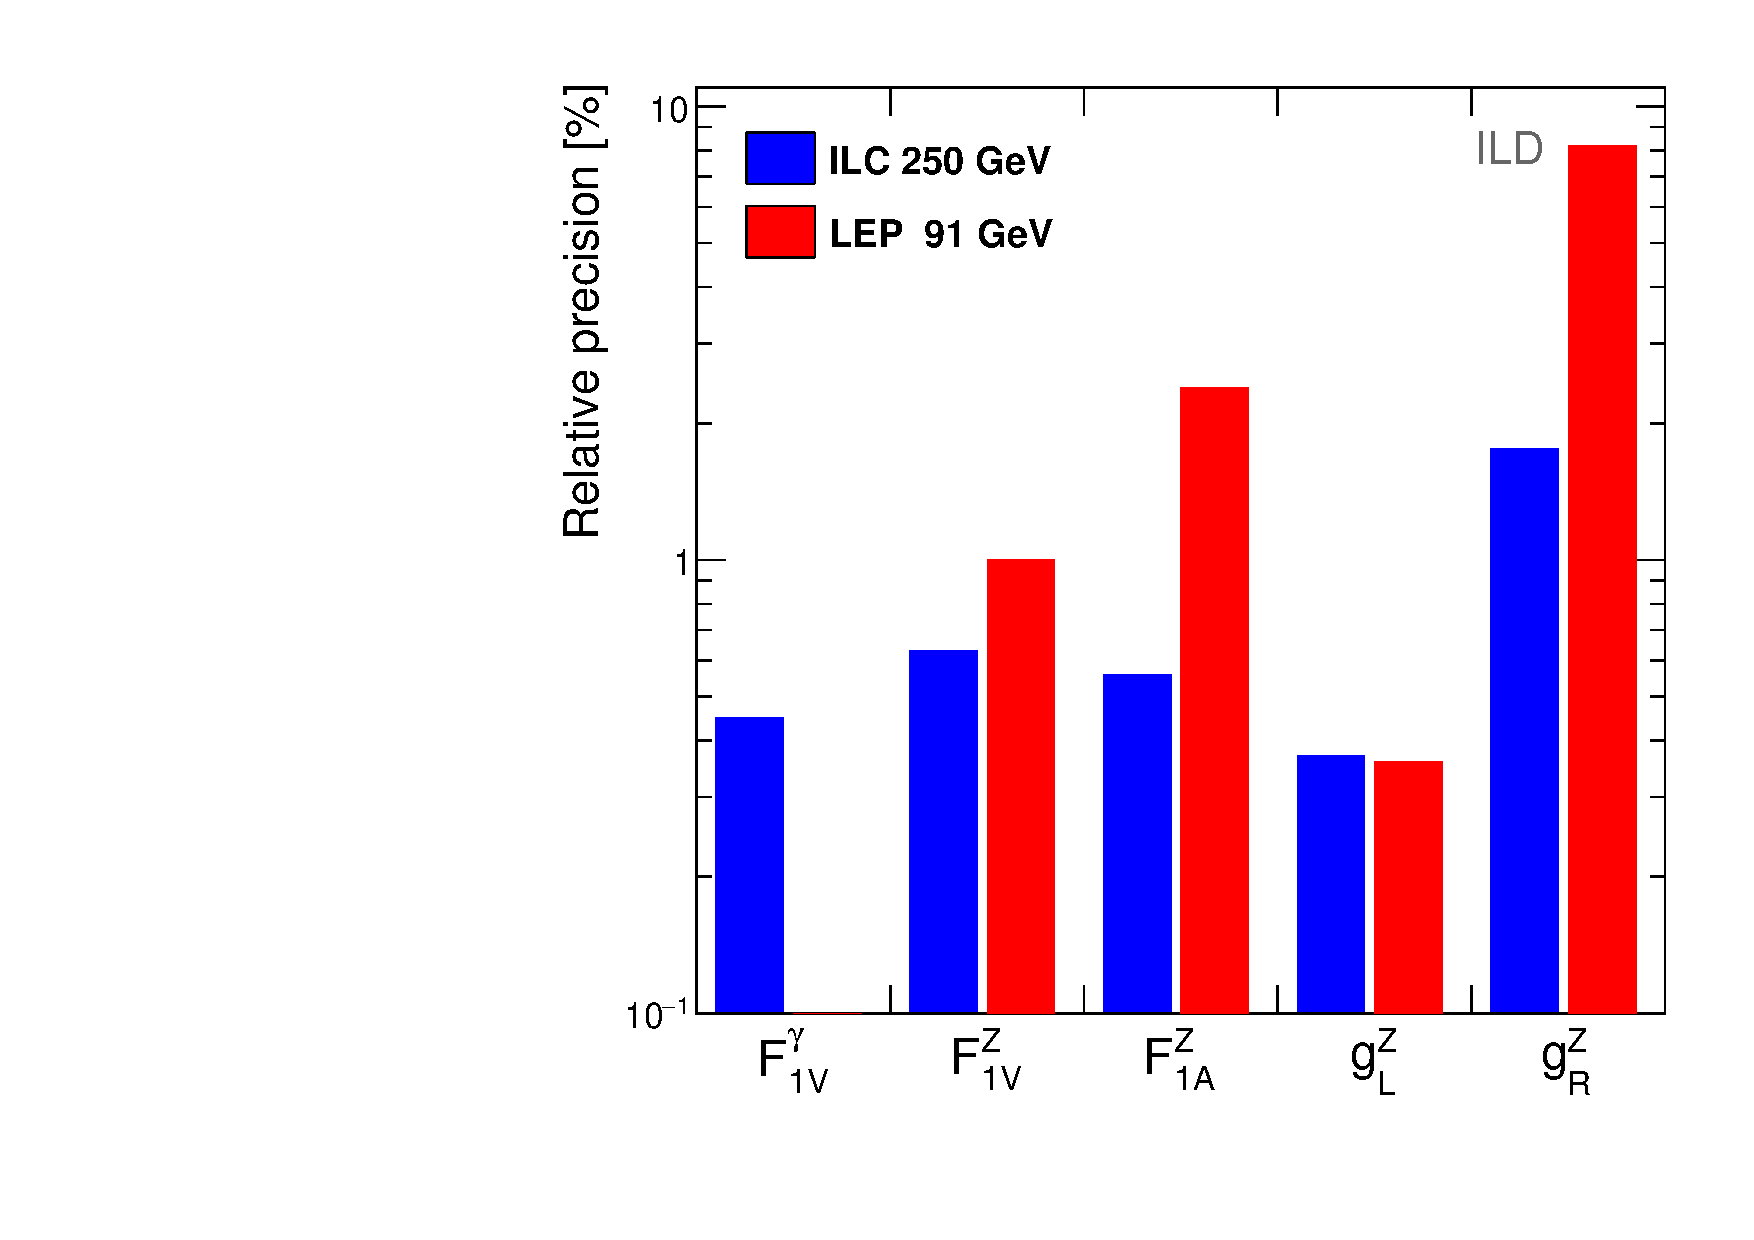
\includegraphics[width=0.45\linewidth]{plots/final-graph-ild.pdf}
	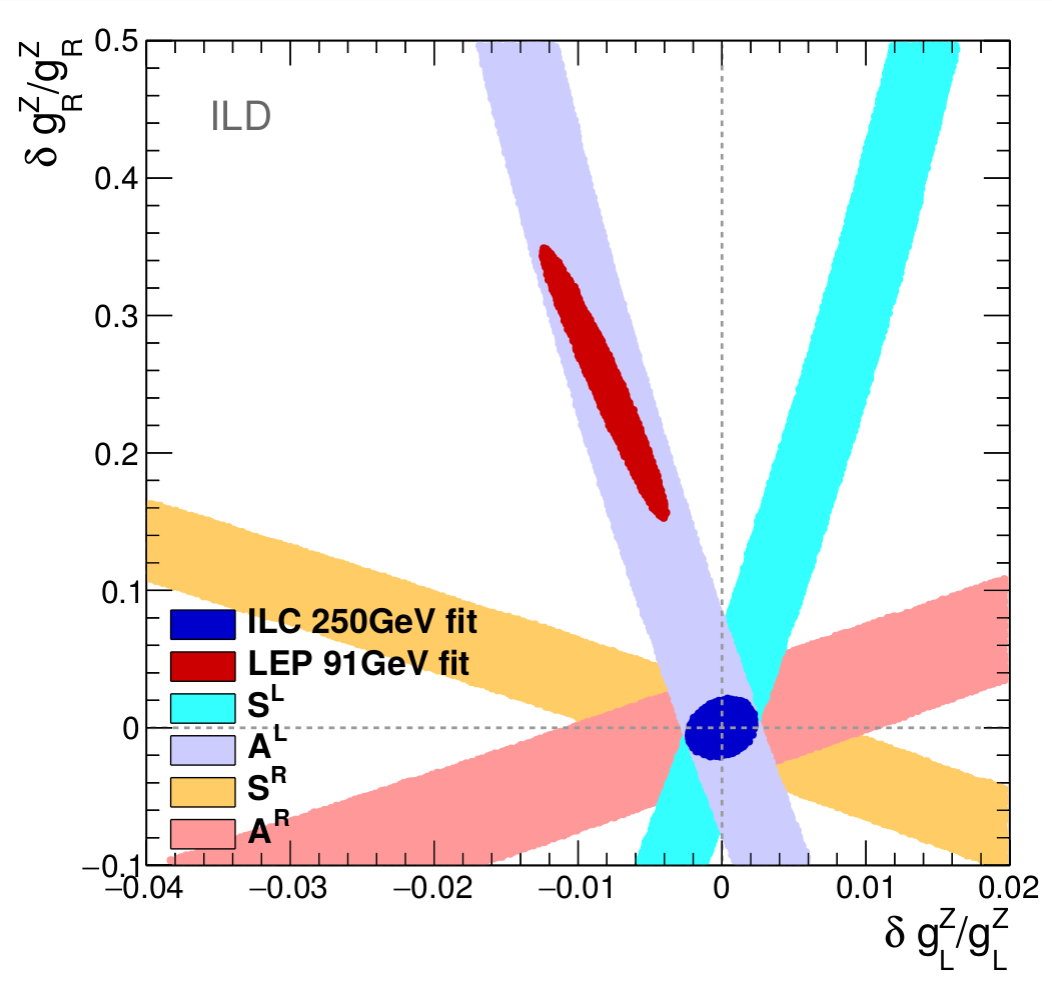
\includegraphics[width=0.45\linewidth]{plots/ilc-precision-ild.png}
	\captionof{figure}{ Comparison of the LEP measurements to the expected precision at the ILC. The results of the ILC assume an integrated luminosity of $\mathcal{L} = 500$\,fb$^{-1}$ shared between beam polarizations at $\sqrt{s} = 250$\,GeV.}
		\label{fig:LEPILCResult_3}
\end{center}\vspace{0.5cm}

%----------------------------------------------------------------------------------------
%	CONCLUSIONS
%----------------------------------------------------------------------------------------

\color{Blue} % SaddleBrown color for the conclusions to make them stand out

\section*{Conclusions}

\begin{itemize}
\item The developed procedure of the b-quark charge reconstruction allows for measuring the b-quark polar angle. The residual impurity is corrected by a data-driven procedure;
\item The b-quark polar angle fit allows for an independent determination of four electroweak couplings of the b-quark. The fit can be extended to include also a term proportional to $\sin^2\theta$, giving access to an independent determination of the tensorial couplings;
\item  The relative precision on the right-handed coupling $dg^Z_R/g^Z_R\approx 2$\% at the ILC is sufficient to confirm at $>5\,\sigma$ or to discard the LEP~I effect, which is at the 25\% level;
\item A reach of $\Lambda \approx 10$\,TeV is achievable for indirect New Physics searches.
%\item The statistical precision after the first $\sqrt{s} = 250\,$GeV ILC program will be almost 5 times better than at LEP;
\end{itemize}

\color{DarkGreen} % Set the color back to DarkSlateGray for the rest of the content

%----------------------------------------------------------------------------------------
%	FORTHCOMING RESEARCH
%----------------------------------------------------------------------------------------

%\subsection*{Forthcoming Research}
%The b-quark charge technique was originally developed for the t-quark polar angle measurement in the semileptonic decay channel and it can be applied to the fully hadronic $t\bar{t}$ decays.
%The kaon charge method can be extended on the c-quark polar angle analysis, where one can improve the LEP~I results on the c-quark couplings precision. 
%Hence, at the ILC one can measure the top, bottom and charm quark electroweak couplings with an excellent sensitivity to New Physics effects.

\subsection*{Acknowledgements}

These studies are done using the full ILD simulation and we acknowledge the work of the ILD software and simulation groups.
 %----------------------------------------------------------------------------------------
%	REFERENCES
%----------------------------------------------------------------------------------------
\titleformat{\section}
{\normalfont\fontsize{30}{15}\bfseries}{\thesection}{1em}{}

\color{DarkSlateGray}
\small
%\nocite{*} % Print all references regardless of whether they were cited in the poster or not
\bibliographystyle{unsrt} % Plain referencing style
\bibliography{../mainbib} % Use the example bibliography file sample.bib

%----------------------------------------------------------------------------------------
%	ACKNOWLEDGEMENTS
%----------------------------------------------------------------------------------------

%\section*{Acknowledgements}

%Etiam fermentum, arcu ut gravida fringilla, dolor arcu laoreet justo, ut imperdiet urna arcu a arcu. Donec nec ante a dui tempus consectetur. Cras nisi turpis, dapibus sit amet mattis sed, laoreet.
